
The \bbonu decay half-life has been introduced in Eq.~\eqref{eq:Tonu} for a decay mediated by the exchange of light neutrinos. We recover the standard definition of the nuclear matrix element (NME) by factoring out the hadron coupling, $g_A$~\cite{Engel:2016xgb,Agostini:2022zub},
\begin{align}
T_{1/2}^{-1} =  G^{0\nu}\left(Q,Z\right)\,g_A^4\,\left(M^{0\nu}_\text{light}\right)^2\,m^2_{\beta\beta}\,,
\label{eq:master}
\end{align}
where $M^{0\nu}_\text{light}$ emphasizes that this NME only corresponds to the many-body part and to light-neutrino exchange\footnote{In eq.~\ref{eq:master}, the term $G^{0\nu}$ is expressed in yr$^{-1}\cdot$eV$^{-1}$ units. Alternatively, this equation is often written dividing $m^2_{\beta\beta}$ by the electron mass squared. In the latter case, $G^{0\nu}$ would have yr$^{-1}$ units.}.
As discussed in Sec.~\ref{sec:bb0nu}, the half-life necessarily depends on an unknown parameter that describes the mechanism beyond the standard model of particle physics responsible for the violation of lepton number in the decay, that is, for the creation of matter without antimatter. In the light-neutrino exchange scenario, this parameter is $m_{\beta\beta}$, as illustrated in Eqs.~\eqref{eq:Tonu} and~\eqref{eq:master}. Therefore, as discussed in Sec.~\ref{subsec:bb0nu_lightmajoranaexchange}, in order to gain information on new physics after the \bbonu-decay discovery, the remaining components of the half-life must be reliably known. Moreover, a good knowledge of these parts allows one to estimate the reach, in terms of the parameter space explored, of experimental proposals targeting a given half-life sensitivity~\cite{Agostini:2021kba}.

The components of the \bbonu-decay rate within the standard model of particle physics in Eq.~\eqref{eq:master} cover the atomic physics related to the emitted electrons ---through the phase-space factor of the transition, $G^{0\nu}\left(Q,Z\right)$--- and the structure of the initial and final nuclear states ---through the NME, $M^{0\nu}_\text{light}$. In addition, $g_A$ represents the hadron coupling of the interaction to nucleons (protons or neutrons), which are the degrees of freedom used by many-body methods to calculate the NMEs.
% , while the fundamental interaction driving the decay happens at the level of quarks and gluons ---the degrees of freedom of the underlying theory, quantum chromodynamics (QCD)---, 
Nonetheless, Eq.~\eqref{eq:master} is a simplification in the sense that various components contribute to $M^{0\nu}_\text{light}$, and they appear associated with different couplings at the nucleon level, not only $g_A$. These aspects are explained in detail in Sec.~\ref{subsec:nme_parts}.

\begin{figure}[t]
	\begin{center}
	\includegraphics[width=\textwidth]{img/g0nu.png} 	\caption{Phase-space factors $G^{0\nu}$ appearing in eq.~\ref{eq:master}, for all 11 \bb emitters with \Qbb$>2$~MeV. Values taken from \cite{Kotila:2012zza}.
 \label{fig:phase_space}}
	\end{center}
\end{figure}

Phase-space factors are quite accurately known for all relevant nuclei used in \bbonu decay experiments~\cite{Kotila:2012zza,Stoica:2013lka}. Figure~\ref{fig:phase_space} shows the corresponding values for the light-neutrino exchange mechanism.
In contrast, despite recent progress, NMEs and some of their associated hadron couplings are still poorly known. In the remaining of this section we discuss the structure of the NMEs to be calculated as well as their corresponding couplings. Further, we briefly detail the many-body methods used to calculate NMEs and how to test the quality of the calculations. Finally, we review the status of NME predictions, including efforts to quantify their theoretical uncertainties.

\subsection{Nuclear matrix elements: long- and short-range parts}
\label{subsec:nme_parts}

The \bbonu decay of a nucleus is a second order process. Therefore, the standard derivation of the \bbonu decay half-life builds on the one-body weak currents~\cite{Doi:1985dx,Tomoda:1990rs,Engel:2016xgb}. For leptons the current reads
\begin{equation}
j_{L\mu}=\overline{e}\gamma_{\mu}\left(1-\gamma_{5}\right)\nu_{eL}, \qquad \nu_{eL}=\sum_{i}U_{ei}\nu_{iL}\,,
\label{eq:j_mu}
\end{equation}
while for hadrons it is
\begin{align}
J_{L}^{\mu\dagger} = \langle  p \rvert\, \tau^{-}
\left[\frac{}{}g_{V}(p^{2})\gamma^{\mu}
+ig_{M}(p^{2})\frac{\sigma^{\mu\nu}}{2m_{N}}p_{\nu}
-g_{A}(p^{2})\gamma^{\mu}\gamma_{5}
-g_{P}(p^{2})p^{\mu}\gamma_{5}
\right] \lvert n \rangle.
\label{eq:J_mu}
\end{align}
Nucleons in nuclei are nonrelativistic, and therefore the one-nucleon current can be expanded to
\begin{align}
J^0_{L,1}=&\left[g_V(p^2)\right]\tau^-_1\,, \nonumber \\
\bm{J}_{L,1}=&\left[
g_A(p^2) {\bm \sigma}_1
-g_P(p^2)\frac{{\bm p}\left({\bm p}\cdot{\bm \sigma}_1\right)}{p^2+m_{\pi}^2}
+ig_M (p^2)\frac{{\bm \sigma}_1\times{\bm p}}{2m_N}
\right]\tau^-_1\,,
\label{eq:J_nonrel}
\end{align}
where the vector coupling $g_V(0)=1$ is responsible for Fermi-type $\beta$ decays and the axial coupling $g_A(0)=1.27$ drives Gamow-Teller $\beta$ decays. For \bbonu decay, it is important to take into account the momentum transfer dependence of these couplings, usually parameterized as a dipole, $g_{A/V}(p^2)=g_{A/V}(0)/(1+p^2/\Lambda_{A/V}^2)^2$, with $\Lambda_{A/V}\simeq 1$ GeV. The pseudoscalar term is also quite relevant, because its coupling, assuming the Goldberger-Treiman relation, is $g_P(p^2)=g_A(p^2)$ neglecting corrections of about 1\%. The smallest contribution comes from the magnetic coupling term, with $g_M(0)=4.71$. This term is usually regularized also with a dipole with parameter $\Lambda_V$.

However, nucleons are composite particles of quarks and gluons, the fundamental degrees of freedom of the underlying theory of the strong force, quantum chromodynamics (QCD). Therefore, two-nucleon currents are needed to complement the one-nucleon one in Eq.~\eqref{eq:J_nonrel}. Two-body currents introduce the coupling of an external probe to two interacting nucleons. Even though they have been recognized for several decades, the relevant two-nucleon diagrams and the value of the corresponding couplings remained with large uncertainties~\cite{Brown:1987obh,Towner:1987zz}, until recently.

A key step forward arrived with the development of chiral effective field theory (EFT), an effective theory of QCD valid at nuclear structure energies and momenta of the scale of the pion mass, $m_\pi$~\cite{Epelbaum:2008ga}. Chiral EFT provides a systematic expansion of nuclear forces~\cite{Machleidt:2011zz,Hammer:2012id} in terms of nucleons interacting via pion exchanges ---the physics included explicitly in the EFT--- and contact interactions  ---which encode the unresolved high-energy physics. Likewise, chiral EFT provides an expansion for the interaction of nucleons with external probes, in particular via the vector and axial currents that enter the weak interaction. Chiral EFT currents also involve pion exchanges and contact interactions. The top diagrams in Fig.~\ref{fig:currents} show the leading one-nucleon currents, which include the leading $g_V$ and $g_A$ terms (top left diagrams) and the $g_P$ one (top right diagram). These three contributions appear at leading order in chiral EFT. This is consistent with their similar importance for processes with $p\sim m_{\pi}$ in Eq.~\eqref{eq:J_nonrel}. The magnetic term appears at higher order in chiral EFT, which explains why this term is numerically smaller than the rest in Eq.~\eqref{eq:J_nonrel}.

\begin{figure}[t]
	\begin{center}
		\includegraphics[width=0.16\textwidth]{img/1bc.eps} \hspace{1cm}
			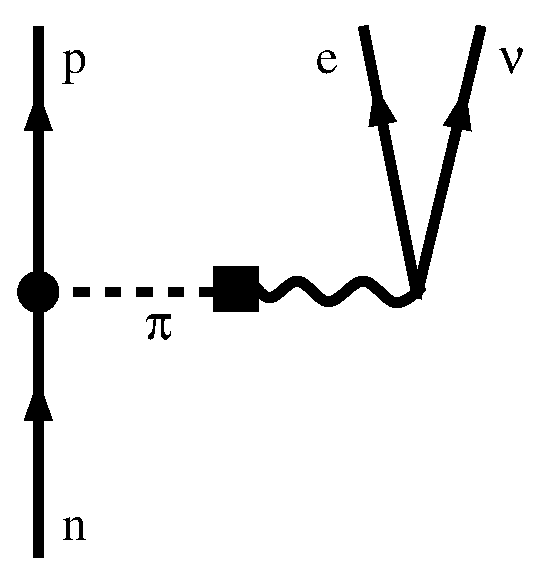
\includegraphics[width=0.22\textwidth]{img/1bc_pion.eps} \\ \vspace{0.5cm}
			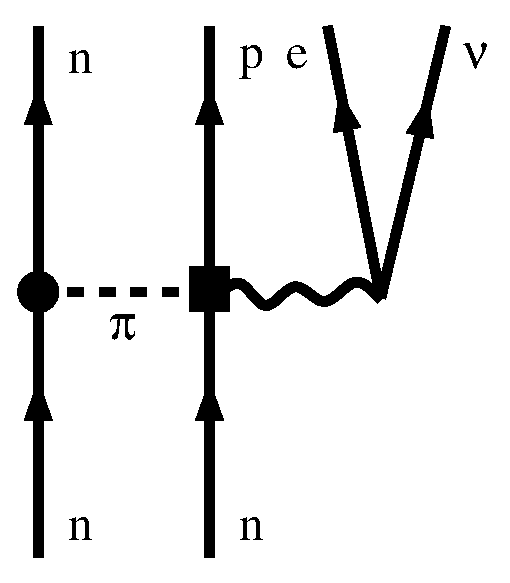
\includegraphics[width=0.22\textwidth]{img/2bc_long.eps} \hspace{.2cm}
			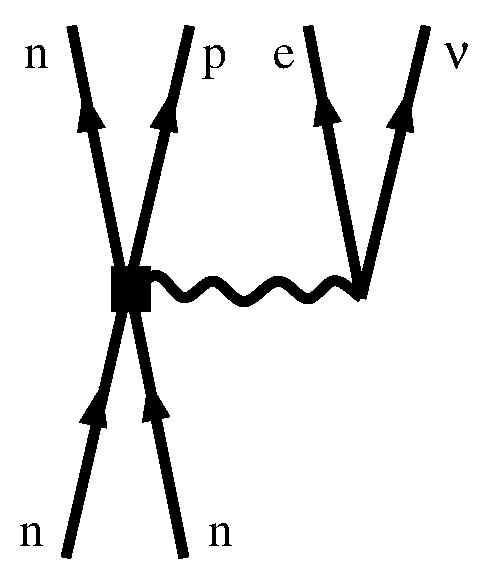
\includegraphics[width=0.21\textwidth]{img/2bc_short.eps} \hspace{.2cm}
   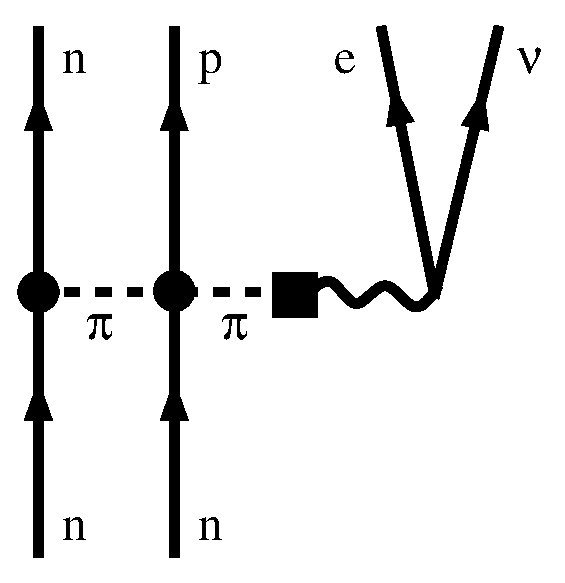
\includegraphics[width=0.245\textwidth]{img/2bc_long_pion.eps}
   \hspace{.2cm} 
   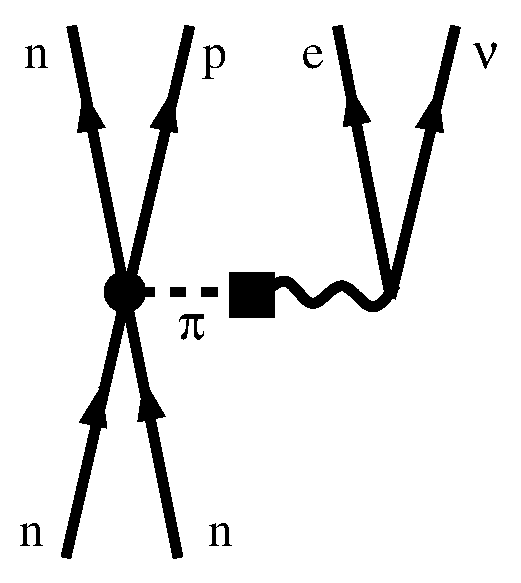
\includegraphics[width=0.225\textwidth]{img/2bc_short_pion.eps}
		\caption{Diagrams for one-nucleon weak-interaction currents (top) and leading two-nucleon weak-interaction currents (bottom). Solid lines represent nucleons, dashed lines indicate pions, and wavy lines the mediator ($W$ boson). In all cases, only one nucleon ($n$) turns into a proton ($p$). The currents with mediator coupling to the pion involve finite momentum transfer, and they are negligible for $\beta$ decay but contribute to \bbonu decay. %Vector two-nucleon currents receive contributions from an additional diagram, but they are subleading for \bbonu decay.
  \label{fig:currents}}
	\end{center}
\end{figure}

In addition, chiral EFT predicts the leading two-nucleon diagrams that correct one-nucleon currents, indicated in the bottom part of Fig.~\ref{fig:currents}. For \bbonu decay, the leading two-nucleon current is the axial one, given by~\cite{Park:2002yp,Krebs:2016rqz,Baroni:2015uza}
\begin{align}
\label{eq:axial2bc}
\bm J_{A,12} &= -\frac{g_A}{F^2_\pi} \, [\tau_1\times\tau_2]^-
\biggl[ 
c_4\Bigl(1-\frac{\bm p}{p^2+m_\pi^2}{\bm p\cdot}\Bigr)
(\bm \sigma_1\times\bm k_2)+\frac{c_6}{4}
(\bm \sigma_1\times \bm p) 
%+i \, \frac{{\bm p_1+\bm p}'_1}{4 m_N}
 \biggr]
\frac{\bm \sigma_2\cdot\bm k_2}{m_\pi^2+k_2^2}  \nonumber \\
&-\frac{2g_A}{F^2_\pi} \,\tau_2^-
\biggl[c_3 \Bigl(1-\frac{\bm p}{p^2+m_\pi^2}{\bm p\cdot}\Bigr) \,\bm k_2+2c_1 m_\pi^2 \frac{\bm p}{p^2+m_\pi^2} \biggr]  \, \frac{
	\bm \sigma_2\cdot\bm k_2}{m_\pi^2+k_2^2}  \nonumber \\
&- 2d_1 \,\tau_1^-  \Bigl(1-\frac{\bm p}{p^2+m_\pi^2}{\bm p\cdot}\Bigr)
\bm \sigma_1 +(1\longleftrightarrow2) \nonumber \\
&- 2d_2 (\tau_1\times\tau_2)^- (\bm \sigma_1 \times \bm \sigma_2)
\Bigl(1-{\cdot \bm p}\frac{\bm p}{p^2+m_\pi^2}\Bigr),
\end{align}
where the final and initial momenta of the nucleons are $\bm k_i=\bm p'_i-\bm p_i$, $\bm p = -\bm k_1-\bm k_2$, and $c_i$ and $d_i$ are couplings of the EFT that need to be determined by fitting to data or from lattice QCD calculations. The terms proportional to the $c_i$'s correspond to the pion-exchange nucleon diagrams in Fig.~\ref{fig:currents}, while those with short-range nucleon interactions enter with the $d_i$'s. Since the chiral EFT couplings also drive nuclear forces, once these are fit, the two-nucleon current in Eq.~\eqref{eq:axial2bc} is entirely predicted. In \bbonu, a complication arises because the product of two-body currents leads, in general, to a four-body operator hard to handle in many-body calculations. A simple approximation but accurate in $\beta$ decays~\cite{Gysbers:2019uyb}, consists in normal-ordering the two-nucleon current with respect to a Fermi gas reference state with density $\rho_F$. As a result, one obtains an effective one-nucleon current~\cite{Menendez:2011qq}, which just modifies the axial and pseudoscalar terms in Eq.~\eqref{eq:J_nonrel} with corrections $\delta g_A(p^2,c_i,d_i,\rho_F)$ and $\delta g_P(p^2,c_i,d_i,\rho_F)$ dependent on the chiral EFT couplings~\cite{Hoferichter:2020osn}.



Once the weak currents are known, the standard procedure follows second-order perturbation theory to obtain the \bbonu-decay rate~\cite{Doi:1985dx}. However, this approach misses a relevant contribution only recognized recently, independent to the ones in Eqs.~\eqref{eq:J_nonrel} or~\eqref{eq:axial2bc}. In fact, a chiral EFT analysis shows that, without this additional term, which can be understood as the contribution of high-energy light neutrinos, the decay amplitude is not renormalizable due to the divergences induced by the long-range neutrino potential~\cite{Cirigliano:2018hja}.

\subsubsection{Long-range nuclear matrix elements}

Thus, there are two contributions to the \bbonu-decay rate. First, the usual long-range part~\cite{Engel:2016xgb}
\begin{align}
\label{eq:nme_full}
  \sqrt{\Gamma_{0\nu\beta\beta}} = & m_{\beta\beta}  \cdot \frac{g_A^2}{R} \cdot    \!\int \!d\bm x \!\int \!d\bm y \;L^{\mu\rho}(\bm x, \bm y) 
  \nonumber \\ & \int \!d\bm p\,e^{i\bm p({\bm x -\bm y})}\cdot 
  \frac{R}{g_A^2} \sum_{n,m}
  \langle 0^+_f\rvert
  \frac{{J}_{L,n}^{\mu\dagger} ({\bm x})\;{J}_{L,m}^{\rho\dagger}({\bm y})}{{ p}^2}
  \lvert 0^+_i\rangle,
\end{align}
where $R=1.2A^{1/3}$ and $g_A^2$ are factorized out for convenience, and $L^{\mu\rho}$ represents the electron currents. The second line in Eq.~\eqref{eq:nme_full} defines the usual long-range NME, which can be written as
\begin{align}
\label{eq:nme}
  M^{0\nu}_\text{long} = \frac{R}{g_A^2}\,
  \langle 0^+_f\rvert
  \sum_{n.m}
  \tau^-_m\tau^-_n \frac{2}{\pi}\int \big[
    &j_0(pr)\,h_F(p^2)\,\mathbb{I}+j_0(pr)\,h_{GT}(p^2)\,{\bm \sigma}_n\cdot{\bm \sigma}_m \nonumber \\
    +&j_2(pr)\,h_T(p^2)\,S_{nm}
    \big]\,d p\,
  \lvert 0^+_i\rangle, %\\
\end{align}
with Fermi (F), Gamow-Teller (GT) and tensor (T) spin structures, $S_{nm}=3({\hat r}\cdot{\bm \sigma}_n)({\hat r}\cdot{\bm \sigma}_m)-{\bm \sigma}_n\cdot{\bm \sigma}_n$, $j_l(pr)$ spherical Bessel functions and $r=\lvert{\bm r}_n-{\bm r}_m\rvert$. The $h_\text{spin}(p^2)$ functions for the long-range NME are
\begin{align}
\label{eq:nu_potentials_explicit}
h_{F}(p^2)&=g_V^2(p^2), \nonumber \\
h_{GT}(p^2)&=g_A^2(p^2)\left[1-\frac{2}{3}\frac{p^2}{p^2+m_\pi^2}+\frac{1}{3}\frac{p^4}{(p^2+m_\pi^2)^2}\right]+g_M^2(p^2)\frac{p^2}{6m_N^2}, \nonumber \\
h_{T}(p^2)&=g_A^2(p^2)\left[\frac{2}{3}\frac{p^2}{p^2+m_\pi^2}-\frac{1}{3}\frac{p^4}{(p^2+m_\pi^2)^2}\right]+g_M^2(p^2)\frac{p^2}{12m_N^2}.
\end{align}
The approximate effect of two-nucleon currents using a normal-ordering approximation can be obtained by modifying the above functions with the corrections $\delta g_A(p^2,c_i,d_i,\rho_F)$ and $\delta g_P(p^2,c_i,d_i,\rho_F)$.

\subsubsection{Short-range nuclear matrix elements}

Second, there is a short-range contribution to the light-neutrino exchange NME, with similar form as Eq.~\eqref{eq:nme_full} but without the neutrino propagator, $1/p^2$. This term does not stem from the product of two currents. It leads to a short-range NME with Fermi-type spin form~\cite{Cirigliano:2019vdj}:
\begin{align}
\label{eq:nme_short}
  M^{0\nu}_\text{short} = \frac{R}{g_A^2}\,
  \langle 0^+_f\rvert
  \sum_{n.m}
  \tau^-_m\tau^-_n \frac{2}{\pi}\int
    &j_0(pr)\,h_S(p)\,p^2\,d p\,\mathbb{I}\,
  \lvert 0^+_i\rangle, %\\
\end{align}
where the function $h_S(p)$ is
\begin{align}
\label{eq:nu_potentials_short}
h_{S}(p)&=2\,g^\text{NN}_\nu f(p/\Lambda_S),
\end{align}
with $g^\text{NN}_\nu$ the corresponding hadronic coupling for this term, and $f(p/\Lambda)$ a function with regulator $\Lambda_S$. Notice that $g^\text{NN}_\nu$ enters linearly in Eq.~\eqref{eq:nu_potentials_short}, in contrast to  any other couplings in  Eq.~\eqref{eq:nu_potentials_explicit}. This indicates that the short-range NME cannot be expressed as a product of two currents. Also, the $p^2$ dependence in Eq.~\eqref{eq:nme_short} illustrates the short-range nature of this NME contribution. Overall, the NME for light-neutrino exchange in Eq.~\eqref{eq:master} is
\begin{align}
M^{0\nu}_\text{light}=M^{0\nu}_\text{long}+M^{0\nu}_\text{short}\,.
\label{eq:nme_total}
\end{align}

Unlike other hadron couplings, $g^\text{NN}_\nu$ cannot be obtained from experiment, because this would involve data on a $2n\rightarrow2p+2e$ decay, or an equivalent process. In principle, the value of the coupling could be extracted from lattice QCD calculations, and efforts in this direction are in progress~\cite{Davoudi:2020gxs,Davoudi:2021noh}. For the time being, approximate QCD results based on dispersion relations~\cite{Cirigliano:2020dmx,Cirigliano:2021qko} and large number of colors~\cite{Richardson:2021xiu} give consistent values for $g^\text{NN}_\nu$ with a reasonable $\sim30\%$ uncertainty. Another strategy is to approximate $g^\text{NN}_\nu$ from the charge-symmetry breaking term of nuclear Hamiltonians~\cite{Cirigliano:2019vdj}. This assumes that the two underlying couplings leading to $g^\text{NN}_\nu$ are the same, as only one of them can be constrained from charge-symmetry breaking.

\begin{figure}[t]
	\begin{center}
	\includegraphics[width=0.65\textwidth]{img/136Xe-QRPA-NSM.pdf}
	\caption{Radial (top panels) and momentum (bottom panels) distributions of the two components of the \bbonu-decay NME in Eq.~\eqref{eq:nme_total}, calculated for $^{136}$Xe. Red (blue) regions represent the long-range (short-range) NME parts. The left panels show results for the QRPA, and right panels for the nuclear shell model (NSM). Figure with results from Ref.~\cite{Jokiniemi:2021qqv}. \label{fig:NME_density}}
\end{center}
\end{figure}

Figure~\ref{fig:NME_density} shows the radial and momentum distributions of the long- and short-range NMEs for the decay of $^{136}$Xe, calculated by the nuclear shell model and quasiparticle random-phase approximation (QRPA) methods fixing $g^\text{NN}_\nu$ from the charge-symmetry breaking of various Hamiltonians. The NME distributions satisfy
\begin{align}
M^{0\nu}_{\text{long/short}}=&\int C_{L/S}(r)\, d r\,, \\
M^{0\nu}_{\text{long/short}}=&\int \widetilde{C}_{L/S}(p)\, d p\,.
\end{align}
The upper panels in Fig.~\ref{fig:NME_density} highlight that the short-range NME distributions, in blue, actually receive contributions from two decaying nucleons at shorter relative distances than the long-range NME ones, shown in red. Consistently, the lower panels in Fig.~\ref{fig:NME_density} reveal that the short-range NME are dominated by larger momentum transfers. Moreover, Fig.~\ref{fig:NME_density} shows that while the short-range NME is generally smaller than the long-range one, it is a sizeable correction, as expected by chiral EFT.




\subsection{Different nuclear structure approaches}
\label{subsec:manybody}

The nuclear structure of the initial and final nuclei in the \bbonu decay plays a relevant role in the value of the NMEs. This is because the relevant momentum transfers in \bbonu decay are of the order $p\sim200$~MeV  ---see Fig.~\ref{fig:NME_density}---, comparable to the Fermi momentum, which sets the typical scale of the momenta of nucleons in nuclei. Therefore, a good description of the initial and final nuclei is a necessary condition in order to get reliable NMEs.

\subsubsection{Tests of nuclear structure calculations and \texorpdfstring{$g_A$}{gA} quenching}

All nuclear many-body methods used to study \bbonu decay make a significant effort to describe with high quality the structure of the initial and final nuclei. In particular, the low-energy spectrum and electromagnetic transitions are typically well described in shell-model~\cite{Menendez:2009xa,Horoi:2015tkc,Iwata:2016cxn,Coraggio:2020hwx,Coraggio:2022vgy,Tsunoda:2023fqw}, energy-density functional theory~\cite{Yao:2021wst}, interacting boson model~\cite{Kotila:2016pib} and QRPA~\cite{Gimeno:2023dxx} calculations, the standard approaches used to calculate NMEs. More recently, {\it ab initio} or first principles methods, discussed in detail in Sec.~\ref{sec:ab_initio}, have also produced NMEs. In medium-mass nuclei, ab initio methods can match the nuclear structure description of the more phenomenological approaches~\cite{Yao:2020olm,Novario:2020dmr,Belley:2020ejd}, while heavier systems are more challenging~\cite{Belley:2020ejd}.
%
Nuclear structure data are very useful to improve many-body calculations, and therefore NME predictions. Notable examples are nucleon-removal and -addition~\cite{Freeman:2012hr,Freeman:2017bak,Szwec:2016fxr} and charge-exchange~\cite{Frekers:2018edj} reactions involving initial and final $\beta\beta$ nuclei. Novel nuclear structure data keep testing calculations. For instance, a recent measurement of the low-energy spectrum of $^{136}$Cs favors particular shell-model Hamiltonians~\cite{Rebeiro:2023kvs}. In addition, correlation between \bbonu-decay and other observables can provide insights to the \bbonu-decay NMEs: good theoretical correlations have been found with double Gamow-Teller~\cite{Shimizu:2017qcy,Yao:2022usd,Jokiniemi:2023bes}, second-order electromagnetic~\cite{Romeo:2021zrn,Jokiniemi:2023bes} and \bbtnu-decay matrix elements~\cite{Jokiniemi:2022ayc}.

However, most calculations systematically overestimate $\beta$-decay Gamow-Teller matrix elements. This puzzle is sometimes coined as {\it $g_A$ quenching}, because matrix elements enter the half-life multiplied by the coupling $g_A$,
\begin{align}
\left(T_{1/2}^\beta\right)^{-1} =  G_{\beta}\left(g_A\,M^{\beta}_{GT}\right)^2\,,
\label{eq:beta}
\end{align}
and the disagreement could also be solved by a reduced $g_A$ value. Fortunately, a simple correction to the $\beta$-decay matrix elements suffices to reach good agreement with data. In shell-model calculations for nuclei with mass number $A\sim10-50$, the matrix-element reduction is captured by constant {\it quenching} factors $q\sim 0.7-0.8$~\cite{Chou:1993zz,Wildenthal:1983zz,Martinez-Pinedo:1996zvt}. Once this factor is known from $\beta$ decays, calculated Gamow-Teller strength distributions agree well with measured values from charge-exchange reactions. Moreover, shell-model half-life predictions for the \bbtnu decay of $^{48}$Ca~\cite{Caurier:1990dc,Poves:1995rg} and the $2\nu$ double-electron capture of $^{124}$Xe~\cite{CoelloPerez:2018ghg} anticipated the subsequent measured values~\cite{Balysh:1996vr,XENON:2019dti}. The interacting boson model and QRPA also overestimate Gamow-Teller matrix elements~\cite{Barea:2015kwa,Pirinen:2015sma}. The latter, however, by an amount depending on the strength of the proton-neutron pairing interaction used.

Nonetheless, the phenomenological quenching correction, while useful, does not pinpoint the origin of the deficiency in the many-body calculations. A proper answer is given by ab initio methods. These approaches describe the low-energy properties of light systems with $A\lesssim 14$ extremely well, including $\beta$-decay half-lives without any adjustments~\cite{Pastore:2017uwc,Gysbers:2019uyb}. There are two main aspects that ab initio methods incorporate, but others do not: first, additional nuclear correlations due to the more sophisticated many-body approach; second, two-nucleon currents, introduced in Sec.~\ref{subsec:nme_parts}. In $A\lesssim 14$ nuclei, nuclear correlations are the main aspect to describe well $\beta$ decays~\cite{Pastore:2017uwc,King:2020wmp}, while in heavier systems with $A\sim50-100$~\cite{Gysbers:2019uyb}, both nuclear correlations and two-nucleon currents are needed to reproduce data without any quenching factor. Due to their ability to capture complex correlations and the successful description of $\beta$ decays, ab initio methods promise reliable \bbonu NMEs.

\subsubsection{Ab initio methods}
\label{sec:ab_initio}

Ab initio or first principles nuclear structure studies have experienced an exponential boost over the last decade~\cite{Hergert:2020bxy,Ekstrom:2022yea}. In contrast to other many-body approaches which have some phenomenological components, ab initio methods consider all nucleons in the nucleus and use unadjusted nuclear Hamiltonians ---in most cases derived  from chiral EFT. Moreover, the calculations are systematically improvable and the convergence of the results can be checked explicitly.

Since \bbonu searches focus on relatively heavy isotopes, ab initio methods like quantum Monte Carlo or the no-core shell model, whose computational cost scales exponentially with the number of nucleons, are limited to benchmark NMEs in light nuclei not relevant for experiments~\cite{Pastore:2017ofx,Basili:2019gvn,Yao:2020olm}. Nonetheless, benchmarks are key to test other approaches suitable for heavier systems.

Three ab initio methods have been used to study the \bbonu decay of $^{48}$Ca. Two of them are versions of the in-medium similarity renormalization group (IMSRG), which is based on unitary transformations that bring the many-body Schr\"odinger equation to a more convenient form~\cite{Hergert:2015awm}. Operators such as the \bbonu-decay one transform consistently, a feature missed by other many-body methods because of their phenomenological character. The first ab initio NME calculation used the in medium generalized coordinate method (IM-GCM)~\cite{Yao:2020olm}. This variant considers various reference states, as the initial and final \bbonu decay nuclei are different, and then includes additional nuclear correlations, exploring deformation  or proton-nucleon pairing via the GCM.

The second is the related valence-space IMSRG (VS-IMSRG) method, which performs IMSRG transformations that decouple a valence space from the core and high-energy orbitals of the full space~\cite{Stroberg:2019mxo}. That is, the VS-IMSRG transforms the many-body problem into one that can be solved with standard nuclear shell-model techniques, with the advantage that it provides an unadjusted nuclear Hamiltonian and a consistent \bbonu-decay operator.

The third is the coupled clusters (CC) approach, which adds singles (one-particle--one-hole like), doubles (two-particle--two-hole) or triples correlations on top of a reference state, which needs to be a reasonable approximation to the nucleus of study~\cite{Hagen:2013nca}. Only recently, the CC has been extended to deformed nuclei such as $^{48}$Ti, because the breaking of rotational symmetry is computationally expensive~\cite{Novario:2020dmr}.

The IM-GCM, VS-IMSRG and coupled clusters long-range NMEs for $^{48}$Ca agree within the uncertainties of each many-body method (green bands in Fig.~\ref{fig:NME_long}). Moreover, because of the connection to the shell model, the VS-IMSRG predicts NMEs for most relevant $\beta\beta$ nuclei, see Figs.~\ref{fig:NME_long} and~\ref{fig:NME_full}. For these results, the theoretical uncertainties are dominated by the use of various chiral EFT Hamiltonians. Unlike $\beta$-decay calculations, ab initio \bbonu-decay NMEs do not include two-nucleon currents yet, because they are more challenging to implement for finite momentum transfer.

\subsubsection{Many-body approaches for heavy nuclei}
\label{sec:maybody_phen}

\begin{figure}[t]
	\begin{center}
	\includegraphics[width=1.02\textwidth]{img/nme_2023.eps}
	\caption{Comparison of the long-range part of the \bbonu-decay NME for the light-neutrino exchange mechanism, calculated by different many-body methods. For the same method, different symbols indicate results obtained by different groups with different assumptions. Results obtained with energy density functional theory plus the GCM~\cite{Rodriguez:2010mn,LopezVaquero:2013yji,Yao:2014uta} (EDF-GCM, dark blue symbols), the interacting boson model~\cite{Barea:2015kwa,Deppisch:2020ztt} (IBM, cyan bars), the QRPA~\cite{Hyvarinen:2015bda,Simkovic:2018hiq,Mustonen:2013zu,Fang:2018tui,Terasaki:2014rba,Terasaki:2019rbu,Terasaki:2020ndc,Jokiniemi:2022ayc} (orange symbols and red bars), the nuclear shell model~\cite{Horoi:2015tkc,Iwata:2016cxn,Menendez:2017fdf,Horoi:2022ley,Horoi:2023uah,Coraggio:2020hwx,Coraggio:2022vgy,Tsunoda:2023fqw,Jokiniemi:2022ayc} (NSM, gray bars and symbols and black bars), the NSM complemented with the generalized contact formalism~\cite{Weiss:2021rig} (NSM+GCM, brown bars), the IM-GCM~\cite{Yao:2020olm} and VS-IMSRG~\cite{Belley:2020ejd} (dark and light green bars, respectively), the coupled clusters' method~\cite{Novario:2020dmr} (CC, green bar), and an EFT of $\beta$ decay~\cite{Brase:2021uny} (EFT-$\beta$, violet bars). See the text for the differences between the calculations and for an explanation of the error bars of each method. \label{fig:NME_long}}
\end{center}
\end{figure}

Among other methods, the nuclear shell model is one of the main workhorses of nuclear structure~\cite{Caurier:2004gf,Otsuka:2018bqq,Brown:2001zz}. It solves the many-body problem in a configuration space around the Fermi surface, using Hamiltonians with a phenomenological component ---in contrast to the VS-IMSRG.
%, usually limited to the part driving the single-particle physics.
Two strategies quantify shell-model NME uncertainties. First, a statistical variation of all elements of shell-model Hamiltonians to obtain NME density distributions for $^{48}$Ca and $^{136}$Xe~\cite{Horoi:2022ley,Horoi:2023uah} (gray bars in Fig.~\ref{fig:NME_long}). Second, systematic calculations in dozens of nuclei exploiting the correlation between \bbonu and \bbtnu NMEs, and \bbtnu data~\cite{Jokiniemi:2022ayc} (black bars in Fig.~\ref{fig:NME_long}, which include normal-ordered two-body currents). The two \bbonu NME extend the range of previous shell-model NMEs (gray symbols).

A hybrid approach can introduce into the shell model additional correlations captured by more sophisticated ab initio calculations. In particular, the generalized contact formalism~\cite{Weiss:2016obx} combines the short-range correlations captured by the quantum Monte Carlo approach with the shell model~\cite{Weiss:2021rig}. As a result, NMEs are reduced (brown bars in Fig.~\ref{fig:NME_long}) by a larger amount than previous short-range correlations' parameterization~\cite{Simkovic:2009pp}.

The QRPA
%was the first many-body method to describe $\beta\beta$ decays~\cite{Vogel:1986nj,Engel:1988au} and
works in a larger configuration space than the nuclear shell model, albeit with limited nuclear correlations. Most calculations use a spherical QRPA on top of G-matrices~\cite{Hyvarinen:2015bda,Simkovic:2018hiq}, but they can accommodate deformation~\cite{Fang:2018tui} or energy-density functionals~\cite{Mustonen:2013zu}. The QRPA NME uncertainty has been explored with systematic calculations varying the proton-neutron pairing interaction and using the \bbonu-\bbtnu NME correlation~\cite{Jokiniemi:2022ayc} (red bars in Fig.~\ref{fig:NME_long}). The corresponding NME range is smaller than other QRPA values (orange symbols) because of including normal-ordered two-body currents.

Energy-density functional theory combined with the GCM is the other workhorse of nuclear structure studies, especially for heavy nuclei or high-energy excitations~\cite{Paar:2007bk,Robledo:2018cdj}. Different calculations use nonrelativistic~\cite{Rodriguez:2010mn,LopezVaquero:2013yji}
or relativistic~\cite{Yao:2014uta} functionals (dark blue symbols in Fig.~\ref{fig:NME_long}).

The interacting boson model is an algebraic approach assuming nuclei formed by bosons~\cite{Iachello:2006fqa} coupled to different angular momenta. Boson degrees of freedom are then mapped to fermions. For NMEs, the uncertainties explored comprise two interacting boson model Hamiltonians fitted to different properties of the initial and final nuclei~\cite{Barea:2015kwa,Deppisch:2020ztt} (cyan bars in Fig.~\ref{fig:NME_long}).

Finally, \bbonu decay can be studied by a nuclear effective theory for $\beta$ and $\beta\beta$ decays, which considers spherical nuclei with nucleon particles or holes attached~\cite{CoelloPerez:2017xsq,Brase:2021uny}. The coupling of the EFT is fitted using the shell-model \bbonu-\bbtnu NME correlation~\cite{Shimizu:2017qcy}, as the EFT can predict \bbtnu NMEs. The theoretical uncertainties are predicted by the EFT, with the violet bars in Fig.~\ref{fig:NME_long} showing leading-order uncertainties.

\subsection{Nuclear matrix elements with theoretical uncertainties}
\label{subsec:nme_current}

Figure~\ref{fig:NME_long} compares predictions for the long-range part of the \bbonu-decay NME from all nuclear many-body methods discussed in Secs.~\ref{sec:ab_initio} and \ref{sec:maybody_phen}. These sections also explain in detail the meaning of the error bars in Fig.~\ref{fig:NME_long} for each many-body calculation. We note that all theoretical uncertainties are underestimated, being the one for the EFT for $\beta$ decay the one closer to the complete error ---however, these NMEs are also based on shell-model NME correlations, see Sec.~\ref{sec:maybody_phen}.
%This comprises NMEs from several many-body methods beyond the ones available about a decade ago, which limited to the shell model, QRPA, energy-density functional theory and interacting boson model.

Most predicted NME values cluster around $M^{0\nu}_\text{long}\sim1-3$ for the majority of isotopes. These are similar as, or even smaller values than, the lower-end NMEs available a decade ago~\cite{Gomez-Cadenas:2010zcc}, which roughly correspond to the shell-model results in Fig.~\ref{fig:NME_long} (gray symbols and bars). {\it This reduction in the NME values appears because many of the recent calculations address, at least partly, the causes of the $g_A$ quenching in $\beta$ decays}. Therefore, a significant part of the reduction of the NME values due to this issue is expected to be already captured in the NMEs shown in Fig.~\ref{fig:NME_long}.

That is, modern calculations that bring additional aspects, in the form of ab initio NME results (green bars with three different tones), short-range correlations introduced by the generalized contact formalism (brown bars), normal-ordered two-nucleon currents (black and red bars), and the EFT for $\beta$ decay (violet bars) all suggest relatively small NME values. This is especially clear for the $^{48}$Ca long-range NME, where the three different ab initio and several other methods agree within uncertainties. Only energy-density functional GCM and interacting boson results (dark blue symbols and cyan bars) point to relatively large NME values, for $^{48}$Ca and for other isotopes. The latter results, however, may be overestimated because of not including explicit proton-neutron pairing correlations or high-seniority components~\cite{Menendez:2014ena,Hinohara:2014lqa,Menendez:2015kxa}. Some QRPA NMEs without two-nucleon currents (orange symbols) also prefer larger NME values than most many-body methods. 

\begin{figure}[t]
	\begin{center}
	\includegraphics[width=0.8\textwidth]{img/nme_total_2023.eps}
	\caption{Comparison of the full \bbonu-decay NME for the light-neutrino exchange mechanism, calculated with different many-body methods: the QRPA~\cite{Jokiniemi:2022ayc} (red bars), nuclear shell model (NSM, black bars)~\cite{Jokiniemi:2022ayc}, NSM with generalized contact formalism~\cite{Weiss:2021rig} (NSM+GCF, brown bars), VS-IMSRG~\cite{Belley:2023btr} (dark-green bars) and IM-GCM~\cite{Wirth:2021pij} (light-green bar). The color code is the same as in Fig.~\ref{fig:NME_long}. See the text for the differences between calculations and for an explanation of the error bars of each method.\label{fig:NME_full}
	}
\end{center}
\end{figure}

However, Eq.~\eqref{eq:nme_total} indicates that the NMEs shown in Fig.~\ref{fig:NME_long} are only a part of the total NMEs for \bbonu decay mediated by the light-neutrino exchange. Figure~\ref{fig:NME_full} compares the predictions for the total NMEs of the few many-body methods which so far have performed dedicated short-range NME calculations. Like in Fig.~\ref{fig:NME_long}, the total NMEs in Fig.~\ref{fig:NME_full} include part of the causes responsible for the $g_A$ quenching in $\beta$ decays, especially the additional correlations introduced by ab initio methods or the two-nucleon currents included into the shell model and QRPA results.

Light- and dark-green bars in Fig.~\ref{fig:NME_full} show ab initio IM-GCM and VS-IMSRG NMEs, which include nuclear correlations key to reproduce $\beta$-decay data. The small IM-GCM uncertainty bar only takes into account the error due to the short-range coupling $g^{\text{NN}}_\nu$, while the larger VS-IMSRG bars are dominated by the uncertainties due to three nuclear Hamiltonians used. Two of the other results in Fig.~\ref{fig:NME_full} incorporate missing aspects to standard shell-model calculations, either short-range physics via the generalized contact formalism (brown bars) or with normal-ordered two-nucleon currents (black bars). The latter approach has wider uncertainties because it considers $g^{\text{NN}}_\nu$ values from various nuclear Hamiltonians ---this strategy has larger uncertainty than the one used by ab initio methods--- and also because it is based on systematic calculations to gauge statistical shell-model uncertainties. These four calculations give consistent NME values for all available isotopes. The QRPA NMEs (red bars), while generally consistent with other results, extend to larger values and present larger uncertainties. Like in the shell model, these are dominated by systematic calculations to estimate statistical uncertainties and the value of $g^{\text{NN}}_\nu$.

